\chapter{APPLICATIONS TO COVALENTLY BONDED MATERIALS}
\label{ch:pareto_si}

In this chapter, we expand the methdology presented in Chapters \ref{ch:ionic_MgO} and \ref{ch:methodology}.  Here the application of the methodology is applied to develop the Pareto set for the Stillinger-Weber formalism\cite{stillinger1985_sw} for silicon, an archetype for a covalently bonded material system.

\section{Potential Formalism}
Silicon has the electron configuration [Ne]3s2 3p2, which needs four atoms to fill the outer p-orbital and obtain a stable electron configuration.  This is done by forming four sp3-hybridized orbitals which forms strong covalent bonds.  As a result, silicon forms a tetrahedral arrangement with its neighbors, with a strong angular dependency.  To model the angular dependency, the Stillinger-Weber potential\cite{stillinger1985_sw} is a combination of a two-body ($\phi_2$) and three-body ($\phi_3$) terms, which is a function of the interatomic distances ($r_{ij}$,$r_{ik}$) from a central atom $i$ and the angle ($\theta_{ijk}$).
\begin{equation}
    E = \sum_{i<j}\varepsilon \phi_2 (r_{ij})
        +\sum_{j<k}\varepsilon \phi_3 (r_{ij},r_{ik},\theta_{ijk})
\end{equation}
where
\begin{equation}
    \phi_2(r_{ij})=A_{ij} \left[
        B_{ij}
        \left(\frac{\sigma_{ij}}{r_{ij}}\right)^{p_{ij}}
        - \left(\frac{\sigma_{ij}}{r_{ij}}\right)^{q_{ij}}
    \right]
    \exp\left(\frac{\sigma_{ij}}{r_{ij}-a_{ij}\sigma_{ij}}\right)
\end{equation}

\begin{equation}
    \phi_3(r_{ij},r_{ik},\theta_{ijk}) =
        \lambda_{ijk}
        \epsilon_{ijk}
        \left[
            \cos(\theta_{ijk}) - \cos(\theta_{0,ijk})
        \right]
        \exp\left(\frac{\gamma_{ij}\sigma_{ij}}
                       {r_{ij}-a_{ij}\sigma_{ij}}
            \right)
        \exp\left(\frac{\gamma_{ik}\sigma_{ik}}
                       {r_{ik}-a_{ik}\sigma_{ik}}
            \right)
\end{equation}

The $A$, $B$, $p$, and $q$ parameters only apply to the two-body interactions.
The $\lambda$, $\theta_0$ parameters are used only for three-body interactions.
The $\varepsilon$,$\sigma$, and $a$ parameters areshared between the terms.

In order to compare the performance of the potentials, we use the original parameterization of Stillinger and Weber (SW)\cite{stillinger1985_sw}, Vink \emph{et al} (VMWM)\cite{vink2001_sw_Si}, and Pizzagalli \emph{et al} (PG) \cite{pizzagalli2013_sw_Si}.  This information is contained in Table \ref{tbl:sw_parameters_ref}.

\begin{table}[ht]
	\centering
	\caption{Table of parameters for the reference potentials}
	\label{tbl:sw_parameters_ref}
	\begin{tabular}{c c c c}
		\hline
		Parameter & SW & VBWM & PG \\
		\hline
		$\epsilon$ & 2.1686 & 1.64833 & 1.04190 \\
		$\sigma$ &   2.0951 & 2.0951 & 2.128117 \\
		$a$ &       1.80 & 1.80 & 1.80 \\
		$\lambda$ & 21.0 & 31.5 & 31.0 \\
		$\gamma$ & 1.20 & 1.20 & 1.1 \\\
		$A$ & 7.049556277 & 7.049556277 & 19.0 \\
		$B$ & 0.602224558 & 0.6022245584 & 0.65 \\
		$p$ & 4.0 & 4.0 & 3.5 \\
		$q$ & 0.0 & 0.0 & 0.0 \\
		\hline
	\end{tabular}
\end{table}

\section{Methodology}

For the development of a new potential, we use a subset of the reference values from Pizzagalli \emph{et al} \cite{pizzagalli2013_sw_Si} listed in Table \ref{tbl:si_fitting_db}.  These properties include the cohesive energy ($E_c$), the lattice parameter ($a_0$), the four independent components of the elastic tensor for an isotropic material ($C_{11}$, $C_{12}$, $C_{44}$), the bulk and shear modulus ($B$, $G$), and the vacancy formation energy ($E_v$).
These will be referred to as the material properties or the quantities of interest (QOI) and denoted $\bm{q}=(q_1,...q_{N_Q})$ with $N_Q = 7$.
All QOI calculations are unit cell calculation, with the exception of of $E_v$ which uses a $3 \times 3 \times 3$ supercell with a single vacancy.

To calculate the material properties, the software \emph{pypospack} described in Chapter \ref{ch:software} is used to model the vector of parameters $\bm{\theta} = (\theta_1,...,\theta_{N_P})$ as the random variable $\bm{\Theta} = (\Theta_1,...,\Theta_{N_P})$.
Using Monte Carlo sampling techniques, individual random variates are sampled $\bm{\theta} \in \bm{\Theta}$ from the proabability distribution function (PDF) $p_{\Theta}(\theta)$.
\emph{pypospack} evaluates these potentials using either the molecular dynamics code LAMMPS \cite{plimpton1995_lammps} or the lattice dynamics code GULP \cite{gale2003_gulp} to produce the QOI predictions
$\hat{\bm{q}}(\bm{\theta}) = (
    \hat{q}_1(\bm{\theta}),
    ...,
    \hat{q}_{N_Q}(\bm{\theta}))$ for the vector of parameters $\bm{\theta}$.

\begin{table}[htbp]
	\centering
	\caption{Fitting database for Si, reference values taken from Pizzagalli \emph{et al}\cite{pizzagalli2013_sw_Si}}
	\label{tbl:si_fitting_db}
	\begin{tabular}{c c c c}
		\hline
		id & Property & Units & Value \\
		\hline
		$q_1$ & $E_c$     & eV    & -4.63 \\
		$q_2$ & $a_0$     & \AA   &  5.43 \\
		$q_3$ & $C_{11}$ 	& GPa   & 166 \\
		$q_4$ & $C_{12}$  & GPa 	& 64 \\
		$q_5$ & $C_{44}$  & GPa   & 80 \\
		$q_6$ & $B$       & GPa   & 99 \\
		$q_7$ & $E_v$     & eV    & 3.6 \\
		\hline
	\end{tabular}
\end{table}

To assess performance of each potential, the difference between predicted QOI values and their targets is defined as $\bm{\epsilon}(\bm{\theta})=(\hat{\bm{q}}(\bm{\theta})-\bm{q})$.  Ideally  $\bm{\epsilon}(\bm{\theta}) = \bm{0}$, and we can define the potential development problem as a multi-objective optimization problem which minimizes $\bm{L} = (\epsilon_1(\bm{\theta}),...,\epsilon_{N_Q}(\bm{\theta}))$.
Since each objective function in $\bm{L}$ cannot be minimized simultaneously due to performance tradeoffs, the optimization goal is the approximation of the Pareto surface.

To develop an ensemble of potentials, the process outlined in Chapter \ref{ch:methodology} is repeated.  Here the optimization goal is to evolve an initial probability distribution function $p_{\bm{\Theta},0}(\theta)$ to $p_{\Theta^*}(\theta)$, where $\bm{\Theta}^*$ is a random variable, and the individual realizations $\bm{\theta}^*(\omega) \in \bm{\Theta}^*(\Omega)$ is a parameterizaton which produces Pareto optimal performance in predicting $\bm{q}$.

\subsection{Incorporation of Prior Knowledge}

Both in the original SW and the VBWM parameterizations use values of $p=4.0$ and $q=0.0$, while PG looks at a different region of parameter space, where $p=3.5$ and $q=0.5$.
Three different parameter ensembles are calculated: (1) one following the original Stillinger-Weber approach, where $p=4.0$ and $q=0.0$, (2) one using the choice of Pizzagalli, where where $p=3.5$ and $q=0.5$, and (3) one where the $p$ and $q$ are free parameters.
This allows us assess the difference from adding additional free parameters.
Incorporating the ranges of parameterizations from Table \ref{tbl:sw_parameters_ref} to determine the upper and lower bounds for each parameter, the initial probability distribution function to define $\bm{\Theta}_0$ for each approach is defined in Table \ref{tbl:sw_parameters_initial}

\begin{table}[ht]
	\centering
	\caption{Initial proabibilty distribution for parameters.
	         A uniform distribution, $U(a,b)$ with lower bound, $a$, and upper bound, $b$, is used as an uninformative prior distribution.
		 Scalar values indicate equality constraints.}
	\label{tbl:sw_parameters_initial}
	\begin{tabular}{c c c c}
		\hline
		Parameter  & $p=4.0, q=0.0$ & $p=3.5, q=0.0$ & $p,q$ free \\
		\hline
		$\epsilon$ & $U(2.1,2.2)$  & $U(2.1,2.2)$  & $U(2.1,2.2)$ \\
		$\sigma$   & $U(1.0,3.0)$  & $U(1.0,3.0)$  & $U(1.0,3.0)$ \\
		$a$        & $U(1.5,2.0)$  & $U(1.5,2.0)$  & $U(1.5,2.0)$ \\
		$\lambda$  & $U(20,32)$    & $U(20,32)$    & $U(20,32)$   \\
		$\gamma$   & $U(1.0,2.0)$  & $U(1.0,2.0)$  & $U(1.0,2.0)$ \\
		$A$        & $U(6.0,20.0)$ & $U(6.0,20.0)$ &$U(6.0,20.0)$ \\
    $B$        & $U(0.5,1.5)$  & $U(0.5,1.5)$  & $U(0.5,1.5)$ \\
    $p$        & 4.0           & 3.5           & $U(3.0,4.4)$ \\
		$q$        & 0.0           & 0.0           & $U(0.0,1.0)$ \\
    $\cos(\theta_{0ijk})$ & 1/3 & 1/3 & 1/3 \\
		\hline
	\end{tabular}
\end{table}

\subsection{Evolutionary Optimization Strategy}

An iterative strategy is evolve the random variable $\bm{\Theta}_0(\Omega)$ using the recursive algorithm, defined in Chapter \ref{ch:methodology} and used in Chapter \ref{ch:ionic_MgO} to develop an Buckingham potential for the MgO system.  Since the topics contained this chapter has more probability topics than the previous chapter, we define the process and notation which simplify discussion later in this chapter.

The beginning of each iteration $N$ starts with the definition of a prior distribution $p_{\Theta}(\bm{\theta})$ to define the random variable $\bm{\Theta}_{N}(\Omega)$.  In the first iteration ($N=1$), the prior distribution is defined by a uniform distribution for each of the free parameters (see Table \ref{tbl:sw_parameters_initial}).  For iterations $N>1$, the prior distribution
$p_{\Theta}(\bm{\theta})$ is updated using the optimal parameters set from the previous iteration, $\hat{\bm{\Theta}}_{t-1}^*$ in the kernel density estimate (KDE)\cite{rosenblatt1956_kde,parzen1962_kde}.  The updated prior distribution is
\begin{equation}
  \label{eq:si_updated_prior}
  p_{\Theta_{t}}(\bm{\theta})
  =
  \hat{p} (\bm{\theta}:\hat{\bm{\Theta}}_{t-1}^*)
\end{equation}
with $\hat{p}$ being the KDE.

The notation $\bm{\Theta}$ refers the sequence of independent and identically distributed (IID) samples of $\bm{\theta}(\omega) \in \bm{\Theta}(\Omega)$,
\begin{subequations}
  \begin{align}
     \bm{\Theta}
       &= (\bm{\theta}(\omega_1), ...,\bm{\theta}(\omega_M))
	  \label{eq:si_theta_seq_1} \\
       &= (\bm{\theta}_i,...,\bm{\theta}_M)
	  \label{eq:si_theta_seq_2}
  \end{align}
\end{subequations}
for $M$ samples. The techniques for generating this sequence given the probability distribution $p_\Theta(\bm{\theta})$ is described in Chapter \ref{ch:methodology}.

The predictions of the material properties $\hat{\bm{q}}(\bm{\theta})$ is a deterministic function based upon the random variable $\bm{\theta}(\omega) \in \bm{\Theta}$.  Therefore, we can define random variable $\hat{\bm{Q}}(\Omega)$ as a determistic function of the random variable $\bm{\Theta}(\Omega)$.  For each $\bm{\theta} \in \bm{\Theta}$ determined in Equation \ref{eq:si_theta_seq_2}, we calculate
\begin{equation}
  \hat{\bm{Q}} = (\hat{\bm{q}}(\bm{\theta}_1),...,\hat{\bm{q}}(\bm{\theta}_M)
\end{equation}
using LAMMPS\cite{plimpton1995_lammps} as the external simulation code.  $\hat{\bm{Q}}$ are realizations of random variable $\hat{\bm{Q}}(\Omega)$ which are generated by evaluating each of the random variates $\bm{\theta} \in \bm{\Theta}$ through the $\hat{\bm{q}}(\bm{\theta})$.

In the next step, we define the conditions for optimality by constraining $\hat{\bm{Q}}(\bm{\Theta})$ with two filters $\mathcal{F}_1$ and $\mathcal{F}_2$. A filter $\mathcal{F}$ selects the elments of
$\hat{ \bm{q} }(\bm{\theta}) \in \hat{\bm{Q}}(\bm{\Theta})$
which satisfies the inequality constraints defined in $\mathcal{F}$.  The surviving candidate potentials after the filtration by $\mathcal{F}$ is denoted
$\mathcal{F}(\hat{\bm{Q}}(\bm{\Theta}))$ with
$\mathcal{F}(\hat{\bm{Q}}(\bm{\Theta})) \subseteq \hat{\bm{Q}}(\bm{\Theta})$.  The filters are mutually independent so

The first filter $\mathcal{F}_1$ filters out points which are not Pareto optimal, by removing the dominated points.  The second filter $\mathcal{F}_2$ removes pathological parameterizations.  To identify outliers, we score each potential according to the absolute errors rescaled by the QOI target value, and calculate the scaled distance to the origin
\begin{equation}
  \label{eq:si_outlier_filter}
	d(\bm{\theta})
  =
  \left[
    \sum_{i=1}^{N_Q} \frac{|\epsilon_{i}(\bm{\theta})|^2}
                          {q_i^2}
  \right]^{1/2}
\end{equation}
The determination of the number of potentials to remove is subjective.  If too many potentials are removed, then this filter becomes too aggressive and behaves as a global scalar optimization algorithm to minimize Equation \ref{eq:si_outlier_filter}.  If too many outliers are kept, then variance-covariance matrix used to determine the bandwidth of the kernel density estimator spreads the probability density in pathological directions, increasing the number of samples required to identify new Pareto optimal potentials.  Here 5\% of the worst performing potentials are eliminated defined by Equation \ref{eq:si_outlier_filter}, which appears to be an appropriate value of this problem.

The optimal parameterizations $\bm{\theta}^* \in \bm{\Theta}^*$ produce QOI predictions which satisfiy all constraints.
\begin{equation}
  \hat{\bm{Q}^*(\bm{\Theta}^*)}
  =
  \mathcal{F}_1(\hat{\bm{Q}}(\bm{\Theta}))
  \cap
  \mathcal{F}_2(\hat{\bm{Q}}(\bm{\Theta})).
\end{equation}
When these filters are applied, the resulting set is
\begin{subequations}
  \begin{align}
     \hat{\bm{Q}}^*
       &= (\hat{\bm{q}}^*(\bm{\theta}^*(\omega_j)),
           ...,
           \hat{\bm{q}}^*(\bm{\theta}^*(\omega_M'))
          )
      \label{eq:si_qoistar_seq_1} \\
       &= (\hat{\bm{q}}^*(\bm{\theta}_j),
           ...,
           \hat{\bm{q}}^*(\bm{\theta}_M')
          )
      \label{eq:si_qoistar_seq_2}
  \end{align}
\end{subequations}
Since $\hat{\bm{Q}}^* \subset \hat{\bm{Q}}$, the index variable changes from $i$ to $j$ and the number of samples in $\bm{Q}^*$ is reduced to $M' \leq M$.

The optimal parameters which produce $\bm{Q}^*$ is $\hat{\bm{\Theta}}^*$.  For the iteration $t$, $\hat{\bm{\Theta}}_{N}^*$ now becomes the sample population required to update the prior distribution in Equation \ref{eq:si_updated_prior}, which continues the iteration process.

To speed convergence of $p_{\Theta}(\bm{\theta})$, we add $\bm{\Theta}_{N-1}^*$ and $\bm{Q}_{N-1}^*$ to $\bm{\Theta}_{N}$ and $\bm{Q}_{N}$, respectively.  The length of the sequence is arbitrary, but the use of $10,000$ samples per iteration appears to be a good tradeoff for potentials with tens of parameters.

\section{Results and Discussion}

The Pareto optimization process produces four components at the end of each iteration, $N$.

\subsection{Univariate analysis}
To analyze the performance of our ensemble of potentials, a univariate inspection of the probability density functions for each of the QOIs can provide insight on the performance of the potential formalism.
Figure \ref{fig:Si_qoi_B} shows the evolution of the predicted values of the bulk modulus for Silicon, $B$.  Each curve is a probability distribution for a specific iteration, estimated using a KDE with the bandwidth determined by the Silverman method\cite{silverman1986_kde}.
In early iterations, the uncertainty reduction in predictions is quite large, but in later iterations the estimates for the Pareto optimal ensemble improves, and the probability density function increases around the target value.

\begin{figure}[h]
	\centering
	\includegraphics[width=5in]{chapter8/qoi_plots/Si_dia_B}
	\caption{Evolution of the prediction of the bulk modulus, $B$, for Silicon.}
	\label{fig:Si_qoi_B}
\end{figure}

In a scalar optimization approach, the cost function converges to a local minima.  The region around a local minima is a basin of attraction for a gradient descent approach.  In contrast, the Pareto optimization approach does not look for a single optimal parameterization, but an ensemble of candidate parameters.  Here, each basin of attraction becomes an elevated region of probability density.  These regions of parameterization become apparent upon visual inspection of the QOI predictions.

Figure \ref{fig:Si_qoi_a0}, shows a the probability density plot for the predictions of the lattice parameter, $a_0$.  This distribution is clearly bimodal; the candidate potentials have two peaks, which indicates two regions with an elevated probability of optimal parameterizations.  In this situation, one peak is centered around the target value of $a_0=5.43$ \AA.  Simular to the evolution of predictions for the bulk modulus, initial iterations have a broad proability distribution which indicates a high level of uncertainty, while the later iterations concentrate the predictions. The second peak becomes more pronounced in later iterations, indicating a second population of potentials which predict a lattice parameter of $~5.0$ \AA.  While potential developers are interested in getting the lattice parameters correct, the second peaks contains potentials which are not dominated by the potentials in the first peak.  Since these potentials are Pareto optimal, they must have better predictions with respect to other material properties.

\begin{figure}[h]
	\centering
	\includegraphics[width=5in]{chapter8/qoi_plots/Si_dia_a0}
	\caption{Evolution of the the prediction of the lattice parameter, $a_0$, for Si.}
	\label{fig:Si_qoi_a0}
\end{figure}

Prediction for the cohesive energy $E_c$ of the system shows an atypical distribution; Figure \ref{fig:Si_qoi_E_coh} shows the evolution of those predictions.  In early iterations ($i=1$ and $i=2$), the probability density functiosn resemble a normal distribution with peaks approximately $-4.0$ eV/atom, which is significantly higher than the target value of $-4.63$ eV/atom.  The candidate parameterizations continue to concentrate their probability density into a smaller region, but does so in an unexpected way.  The tail end probabilities continue to reduce markedly, but by the fifth iteration ($i=5$), a probability density function takes a significantly different shape.  Instead of having a peak, there is a region of elevated probability that is relatively constant over the range $-4.5 < E_c < -3.6 $ eV/atom.  At the final iteration ($i=20$), a clear mode develops at $E_c=-4.3$ eV/atom with a shoulder at $E_c=-3.6$ eV/atom.
The distribution of potentials conveys important information to the potential developer; the most likely region to find Pareto optimal parameterization does not correspond with qoi target value.  Choosing high fidelity with respect to cohesive energy means that less candidate potentials are available.

\begin{figure}
	\centering
	\includegraphics[width=5in]{chapter8/qoi_plots/Si_dia_E_coh}
	\caption{Evolution of the prediction of the cohesive energy, $E_c$ for Si.}
	\label{fig:Si_qoi_E_coh}
\end{figure}

\subsubsection{Analysis of Correlation Matrices}

Since we are interested in tradeoffs, an analysis of the correlation for simulated potentials can detect relationships between parameters and QOIs.
Figure \ref{fig:Si_correlation_plots} displays the correlation data for the last iteration of the potential optimization process.
The top row contains the correlation matrices for the parameters produced by the kernel density estimate and estimates of the QOI.
The bottom row contains the correlation matrices for same components after the dominated points are removed.
In this plots, a red shader is used for positively correlated points and blue shader used for negatively correlated components.  As the correlated components becomes stronger, the color becomes more intense.  This allows the quick identification of components which might be of interest.

Correlations are calculated using the Pearson correlation coefficient.\cite{devore2012_probability}
The correlation coefficient ranges from $-1 \leq \rho_{X,Y} \leq 1$ for two variables $X$ and $Y$.  Correlation equal to either $1$ or $-1$ correspond to a bivariate distribution supported by a line.
The Pearson correlation matrix is symmetric since $\rho_{X,Y} = \rho_{Y,X}$.
The Pearson correlation is invariant under transformation of location and scale; the variables $X$  and $Y$ can be transfomed to $X'=a+bX$ and $Y'=a+bY$ with $a,b,c,d \in \mathbb{R}$ and $b,d > 0$ without changing the correlation coefficient.  As a result, analysis of $\bm{\epsilon}(\bm{\theta})$ and $\hat{\bm{q}}(\bm{\theta})$ are identical.
Although loss functions are used for Pareto optimization, the loss of the sign information frustrates statistical analysis.  The absolute error function, $|\epsilon_i(\bm{\theta})|$, reflects negative values back into the positive quadrant, while the squared error function $\epsilon_i^2(\bm{\theta})$ introduces curvilinear relationships which masks linear relationships.

An examination of the parameter correlation matrices show the general trend of tradeoffs in parameters to produce Pareto optimal results as a single scalar value.  As the correlation matrix plot shows, most parameters are weakly uncorrelated with each other.
There is moderate negative correlation ($\sigma_{A,a}=-0.48$) between the $A$ parameter of the pair components and the $a$ parameter of the 3-body term.
There is a strong negative correlation between the $\sigma$ and both $a$ ($\sigma_{\sigma,a}=-0.74$) and $B$ ($\sigma_{\sigma,B}=-.85$).  Increases in $\sigma$ can be compensated by decreases in $B$ and $a$ to keep a potential Pareto optimal.
This leads to $B$ and $a$ being strongly correlated to each other ($\sigma_{B,a}=0.71$), despite the parameters belonging to the pair and 3-body components, respectively.
The removal of dominated points yields the bottom left correlation matrix plot of Figure \ref{fig:Si_correlation_plots}.
Visual inspection of the figure immediately verifies that the relationships are qualitative similar.
The magnitudes of the correlations are quantitatively stable, indicating that the optimization process is converged.

The right columns of Figure \ref{fig:Si_correlation_plots} are the correlation matrix plots for the QOIs.
The top figure is the unfiltered results of the QOIs produced by the KDE of the last iteration, (i.e. $\hat{\bm{q}}(\bm{\theta} \in \bm{\Theta}_{N=20})$).
The bottom figure being the same predictions filtered to remove dominated points and outliers (i.e. $\hat{\bm{q}}(\bm{\theta} \in \bm{\Theta}_{N=20}^*)$).
The visualization of the two figures shows that the underlying structure between the two figures is qualitative different.

The top-right correlation plot in Figure \ref{fig:Si_correlation_plots} illustrates problems with the Pearson correlation coefficient.
Some parameters produced by the PDF, $p_{\bm{\Theta}}(\bm{\theta})$ produce extremely large prediction errors, $\epsilon_i(\bm{\theta})$ to which Pearson’s correlation coefficient is sensitive; the correlation coefficent is also affected by the magnitude of the slope around which points are clustered, by curvature, by the restriction in the range, and by heteroscedasticty (where the variability of one variable is unequal across the range of values of the second).\cite{wilcox2011_estimation_1,wilcox2011_estimation_2}
Igorance of these data points obscures the "true" correlation coeffient ultimate creates misleading results when inferring relationships when analyzing the correlation matrix.  Here, the correlation matrix infers a linear relationship ($rho=1$ or $\rho=-1$) between $C_{11}$ and $C_{12}$, $C_{11}$ and $B$, and $C_{12}$ and $B$.
Since $B$ is calculated from elements in the elastic tensor, the extreme values of $\rho_{C_{11},B}$ and $\rho_{C_{12},B}$ are likely caused by outliers in the prediction in either $C_{11}$, $C_{12}$, or the bivariate predictions of $C_{11}$ and $C_{12}$.

Filtering outliers to remove both non-Pareto optimal points and outliers results in the bottom right correlation plot in Figure \ref{fig:Si_correlation_plots}.  From visual inspection reveals the correlation plots are qualitative different.  This indicates that convergence of the distribution in parameter space does not converge to Pareto optimal predictions in the performance space, and filtering elements of $\bm{q}(\bm{\theta}(\omega) \in \bm{\Theta}(\Omega))$ still contains information which is uncaptured by a kernel density estimate of Pareto optimal components.

Predictions for the cohesive energy $E_c$ and the vacancy formation energy $E_v$ are highly negatively correlated with each other ($\sigma_{E_c,E_v}=-0.96$), but not with any of the other components.  Predictions of the other QOIs are moderately correlated with each other with the exception of two components.  The $C_{11}$ and $C_{12}$ components are uncorrelated ($\sigma_{C_{11},C_{12}}=0.05$).  The predictions of $B$ and $C_{12}$ are highly correlated ($\sigma_{C_{12},B}=0.89$).

\begin{figure}[ht]
  \centering
  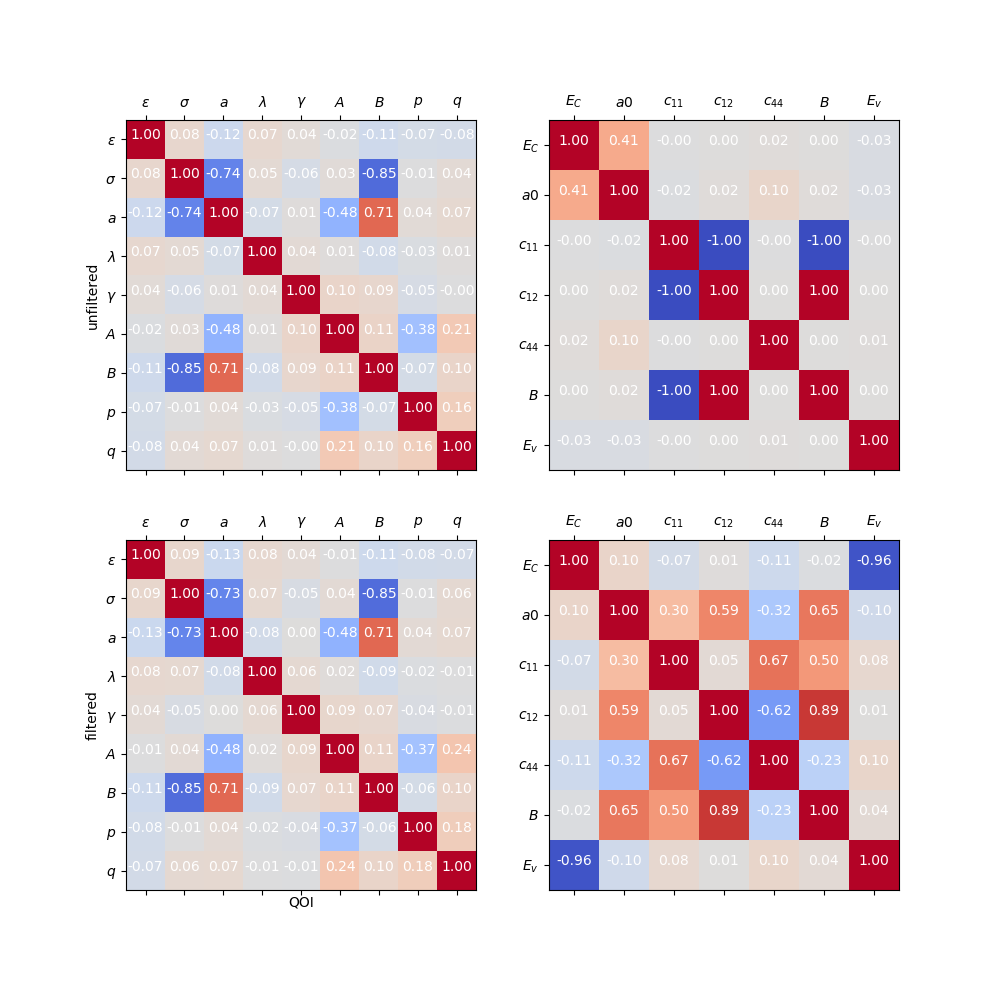
\includegraphics[width=5in]{chapter8/fig_cov_19}
  \caption{A correlation matrix plot with positively correlated variables indicated with a red gradient shader and negatively correlated variables indicated with a blue gradient shader.  Data comes from the $N=20$ iteration.  The left and right columns are the parameters and QOI relationships, respectively.  The top and bottom rows are unfiltered and filtered relationships, respectively.}
  \label{fig:Si_correlation_plots}
\end{figure}

\subsection{Bivariate Analysis}

A non-linear association between may exist between components would not be described by the Pearson correlation coefficient; a property which should evident in this application since each $\hat{q}_i(\bm{\theta})$ is a function of the same realization of the random variable $\bm{\Theta}$.  However, the Pearson correlation coeffient fails to identify anything but linear relationships.  One mechanism to overcome this problem is through the visual inspection of bivariate plots.  In this application, the typical representation of the scattter plot is augmented with a gradient shader to reflect areas of higher density indicated by the kernel density estimate.  The bivariate plot projects the high dimensional space ($N_Q$ for QOI space, and $N_P$ for Parameter space) into the 2-dimensional subspace with basis vectors in the direction of the variables under analysis.  The bivariate scatterplots provide a visual mechanism to identify salient features of the bivariate distribution between two variables, such as curvilinear or multimodal behavior which cannot be captured by correlation statistics.

\begin{figure}[ht]
  \centering
  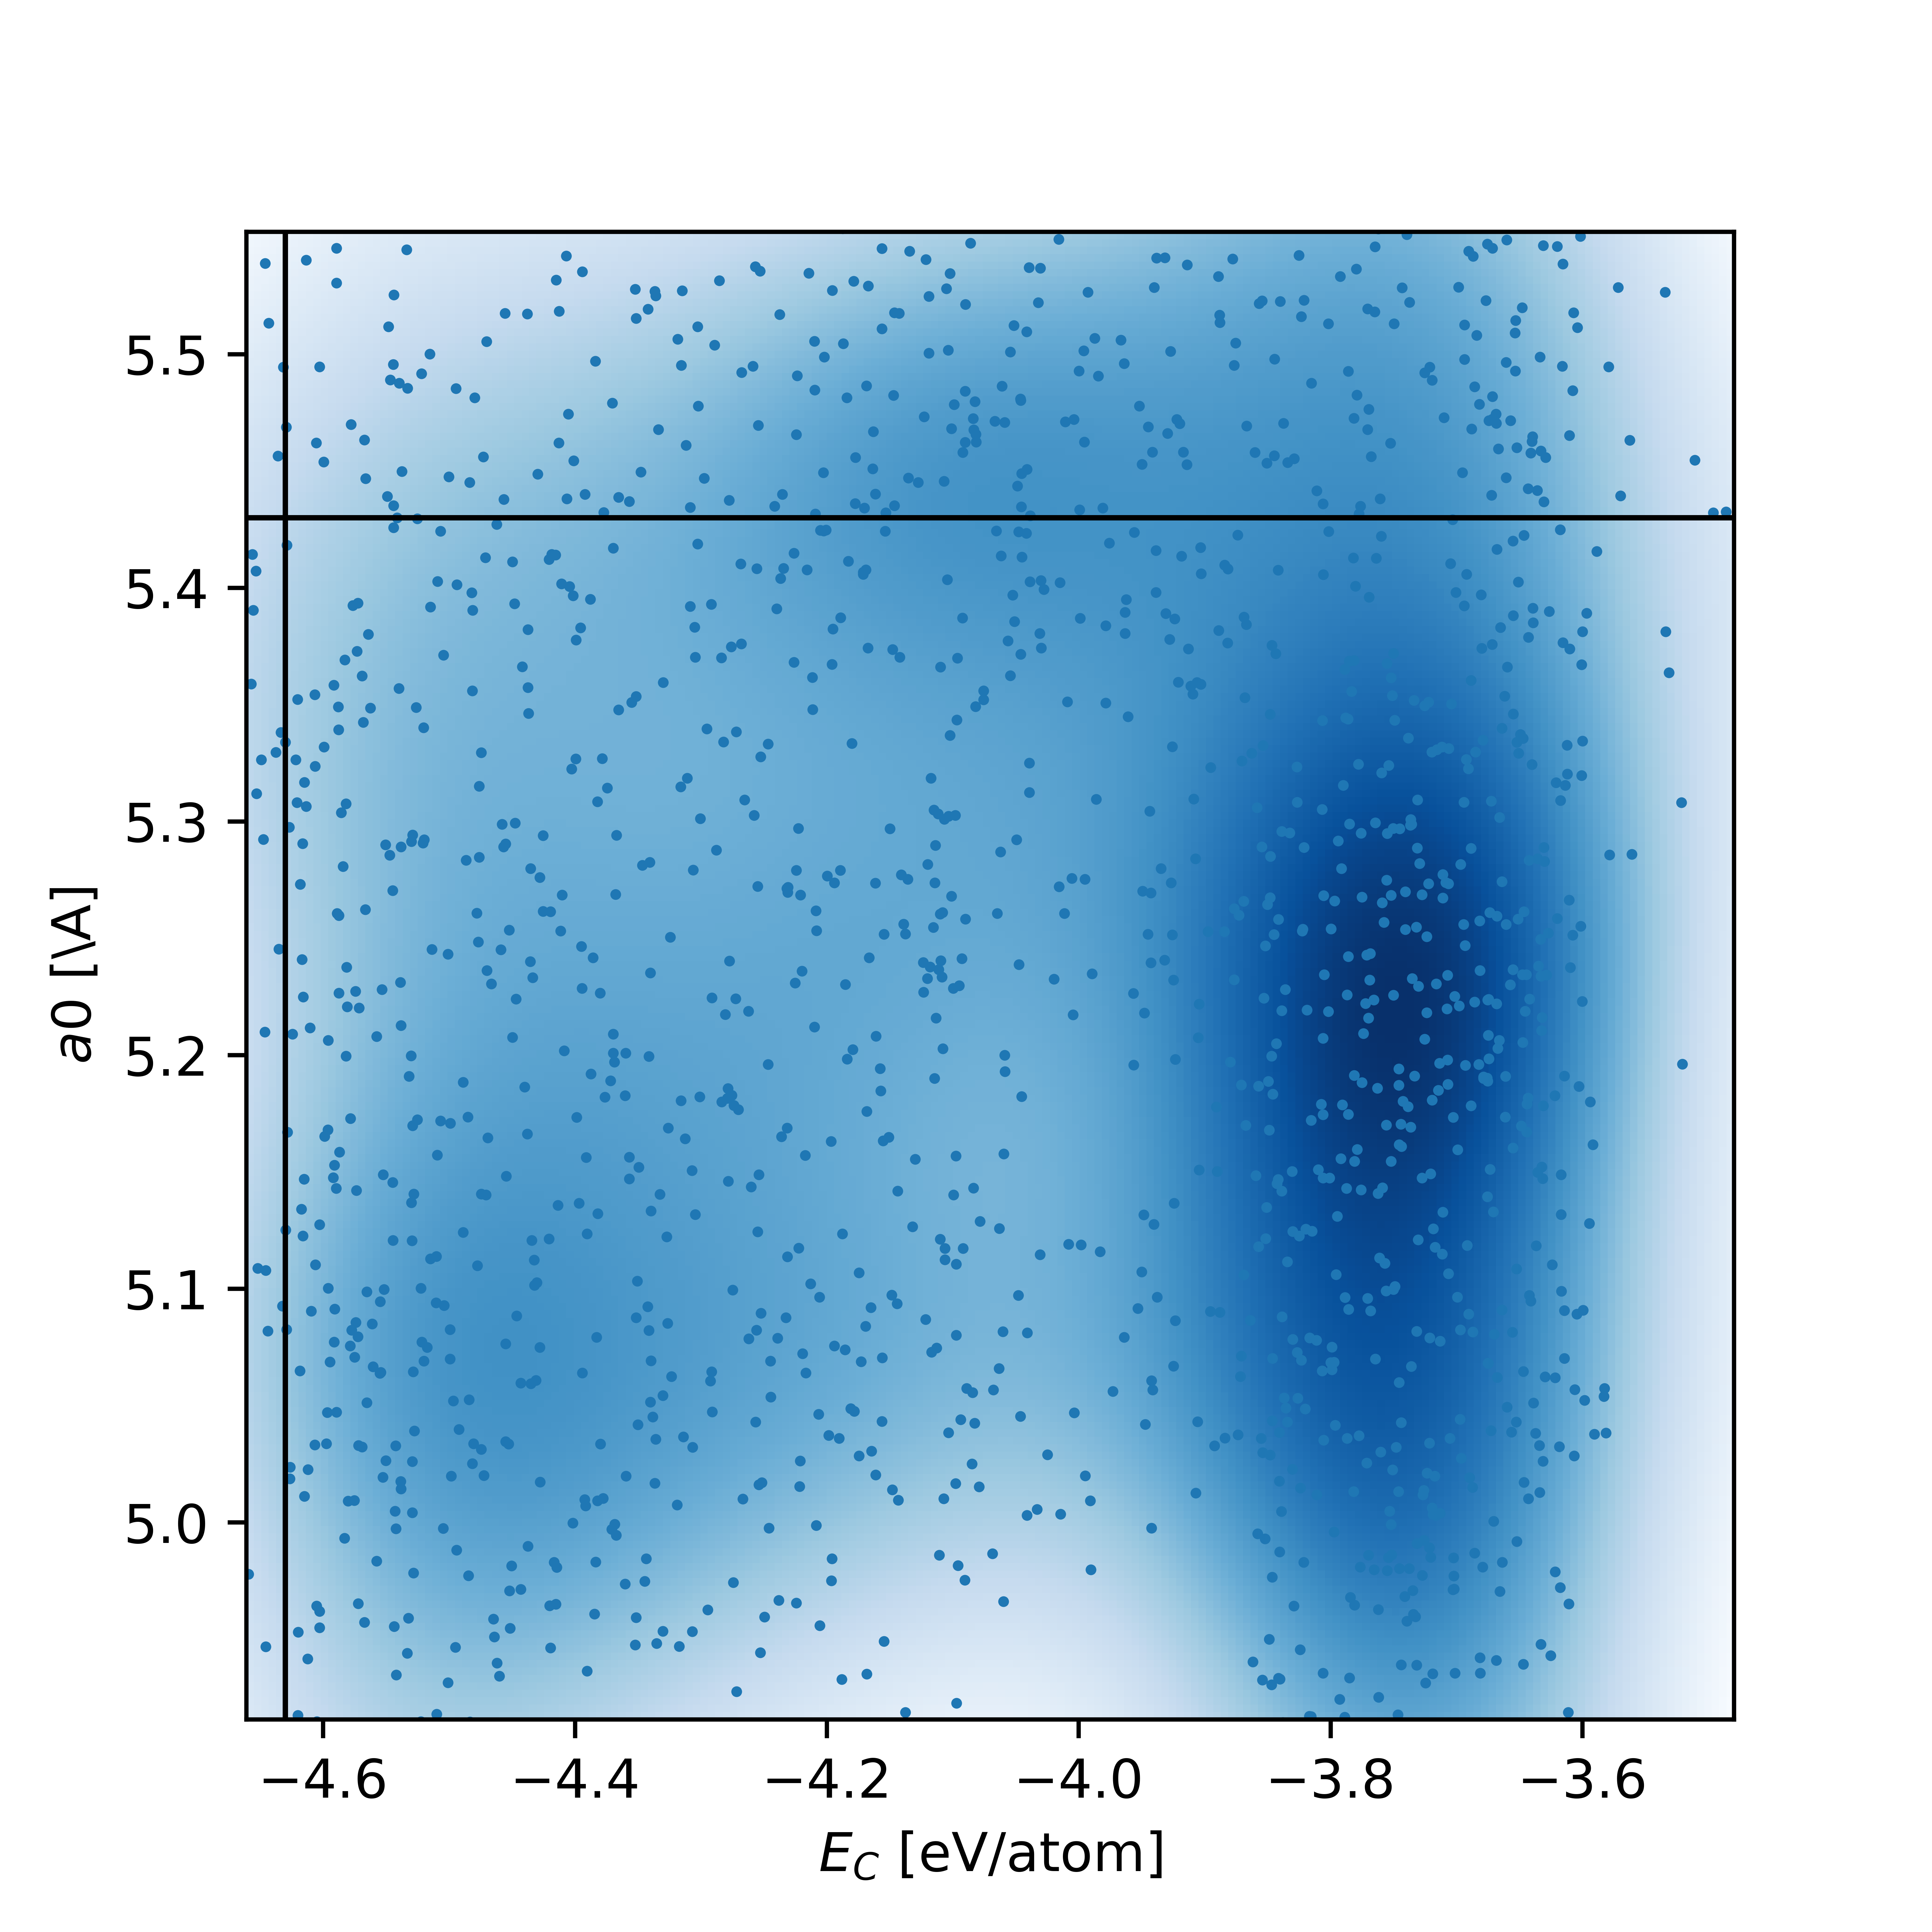
\includegraphics[width=5in]{chapter8/qoi_2d_density_plots/Si_dia_E_coh__Si_dia_a0}
  \caption{A bivariate plot of the predicted values for the cohesive energy $E_c$ against the lattice parameter $a_0$ for Si in diamond phase.  The dark lines indicated the target values for which the potential is optimized against}
  \label{fig:Si_Ec_a0_scatterplot}
\end{figure}

In the development of binary potentials, the predictive performance of the cohesive energy $E_c$ and the lattice $a_0$ are often prioritized.  Unless these material properties are correct, the predictions of material properties for binary system will likely underperform.  For example, poor predictions of lattice paramter leads to artificial strains in the interface of a simulation material, leading to erroneous predictions of surface energies.  In Figure \ref{fig:Si_Ec_a0_scatterplot}, a bivariate plot of the predicted values for the cohesive energy $E_c$ is plotted against the lattice parameter $a_0$ for silicon in diamond phase.
For reference, the target values for each QOI are also indicated on the plot.  Analysis of the bivariate plot indicates a multi modal population with three regions of elevated probability density.
The primary region where of highest density located at $E_c=-3.86$ eV/atom and $a_0=5.22$ \AA, which is the region where most of the Pareto optimal potentials are located.  Two additional regions of elevated density closer to our QOI target values exist.  One closer to the target cohesive energy at $E_c=-4.5$ ev/atom and $a_0=5.05$ \AA.  The other region is closer to the target lattice parameter value at $E_c=-4.1$ eV/atom and $a_0=5.45$ \AA.

This approach is not without drawbacks.  As the number of parameters and the number of QOIs increases, the number of bivariate plots increases expoentially, making the visual inspection of the possible combinations tedious for a complicated potential formalism, which require more QOIs to ensure that the system is not underdetermined.  Adding more elements to system, likewise increases the workload markedly.

In addition, by projecting high dimensional data onto a low dimenstional subspace a causes information loss.  Although we know more parameterizations at a region of elevated density, but we are unable to infer the quality of the simulation with respect to other mmaterial properties.

Finally, this approach is subjective, imprecise, and requires the potential developer to invest a significant amount of time in analysis to partition parameter space to refine the search to a specific area of interest.

\subsection{Gaussian Mixture Models in Two Dimensions}

Now we outline a technique for partitioning the Pareto optimal potentials, into subsets described by a normal distribution using Gaussian mixture models (GMM).  A GMM is a probabilistic model that assumes that all data points are generated from a mixture of a finite number of Gaussian distributions with unknown parameters.  Here we will partition the biobjective space formed by $a_0$ and $E_c$, for GMM analysis.

Before outlining the procedure for Gaussian Mixture Model in the general case, we motivate the use of the algorithm in the 2D case of two QOI variables based upon the previous example of $E_c$ and $a_0$ before moving to a general approach for partitioning the ensemble of Pareto optimal potentials.

A Gaussian mixture model (GMM) is part of the family of a Dirichlet processes, which are a probability distributions whose range are itself a set of probability distributions.\cite{west1994_mixturemodel}
Dirichlet processes are frequently used in Bayesian nonparameteric statistics, where nonparametric does not mean a parameter-less distribution, but rather a model in which the representations grow as more data is observed.  As an example the kernel density estimator is a Dirichlet process; each point has a normal probability density function centered over it.
A GMM with with $K$ components can be written for the random variable $\bm{x}(\omega) \in \bm{X}(\Omega)$ with $\bm{x} \in \mathbb{R}^d$ as the sum of Gaussian distributions,
\begin{equation}
\label{eq:gmm}
  p_{\text{GMM}}(\bm{x}|
                 \bm{\mu}_1,...,\bm{\mu}_K,
                 \bm{\Sigma}_1,...,\bm{\Sigma}_K
                 \phi_1,...,\phi_K)
  =
  \sum_{k=0}^K \phi_k N(\bm{x}|\bm{\mu}_k,\bm{\Sigma}_k)
\end{equation}
where $\bm{\mu}_k$ are the means, $\bm{\Sigma}_k$ is the covariance matrix, $\phi_k$ is the mixing proportion ($0<\phi_k<1$ and $\sum_k \phi_k = 1$), and $N$ is a normal multivariate distribution function with the speciified mean and covariance matrix for the $k$th component of the GMM.

To choose the number of components which should be included in a Gaussian mixture model, we use a method described by Celeux and Soromenho\cite{celeux1996_gmm_components} which selects the number of components through calculation of information criteria (IC).  ICs estimate of the relative quality of statistical models for a given set of data, by penalizing potentials for using a more complicated model.
Here we base the number of clusters based upon the Akaike information criterion (AIC)\cite{akaike1998_aic} and the Bayesian information criterion (BIC) \cite{schwarz1978_bic}.
The AIC or BIC of a model is written in the form $[2\log(\hat{L}+kp]$, where $\hat{L}$ is a likelihood function, $p$ is the number of parameters in the model, and $k$ is $2$ for AIC and $\log(n)$ for BIC.
Given a collection of models for data, both the AIC and BIC estimate the quality of each model relative to the other models, providing a mechanism for model selection.
The \emph{scikit-learn} Python package\cite{pedregosa2011_scikitlearn} is used to fit the GMM for $1 < k < 20$ components and calculate the AIC and BIC with only $E_c$ and $a_0$ provided.
In Figure \ref{fig:Si_Ec_a0_aic_bic}, the BIC indicates that $4$ components should be used in the GMM model, while the AIC indicates are larger number of components should be used.
In a more thorough analysis, GMM models utilizing a number of components from a minimum to a maximum number of components would be examined based upon the different values provided by AIC vs BIC.
\begin{figure}[ht]
	\centering
	\includegraphics{chapter8/aic_bic_plot}
	\caption{Identification of the number of Gaussian components recommmended for a Gaussian mixture model for the biobjective space formed by the lattice parameter $a_0$ and the lattice parameter $a_0$.  Here, the BIC criteria indicates a smaller number of components, while AIC indicates that a larger number of components should be used.}
	\label{fig:Si_Ec_a0_aic_bic}
\end{figure}

The results for the GMM model with $K=4$ components is shown in Figure \ref{fig:Si_Ec_a0_gmm}.  The four different components aree indicated with ellipses and the potential points colored based upon their classification.  The locations of the different normal distributions and their associated weights are listed in Table \ref{tbl:sw_2parameter_gmm}.  In addition to the three clusters which we expected ($k=1,2,3$), a forth cluster ($k=4$) has a large variance which models the outliers.  The orientation of the elipses represents the orientation of the variance-covariance matrix, $\bm{\Sigma}_k$.
The centroid of the elipses for cluster $k$ is specificed by $\bm{\mu}_k$.  The length of the major and minor axis comes from a the eigenvalue-eigenvector decomposition of $\bm{\Sigma}_k$, a process known as principle components analysis (PCA).\cite{pearson1901_pca,hotelling1933_pca}.  The eigenvalues give the length of the major and minor axis and the associated eigenvectors provide the direction.  Since the eigenvetors are orthgonal to each other, PCA is a change of coordinates of the $\bm{\Sigma}$ so that linear vectors (the principle components) describe the orientation of the variance.

\begin{table}[ht]
	\centering
	\caption{Location information for each cluster, $k$  from a two dimensional GMM model consisting of the $E_c$ and $a_0$ components along with weighting $\phi$.}
	\label{tbl:sw_2parameter_gmm}
	\begin{tabular}{c c c c}
    \hline
    $k$ & $\phi$ & $E_c$ & $a_0$ \\
        &        & [eV]  & \AA   \\
    \hline
    1 & 0.28 & -3.72  & 5.12 \\
    2 & 0.36 & -4.43  & 5.18 \\
    3 & 0.27 & -3.93  & 5.38 \\
    4 & 0.08 & -4.09  & 5.34 \\
    \hline
  \end{tabular}
\end{table}

\begin{figure}[ht]
	\centering
	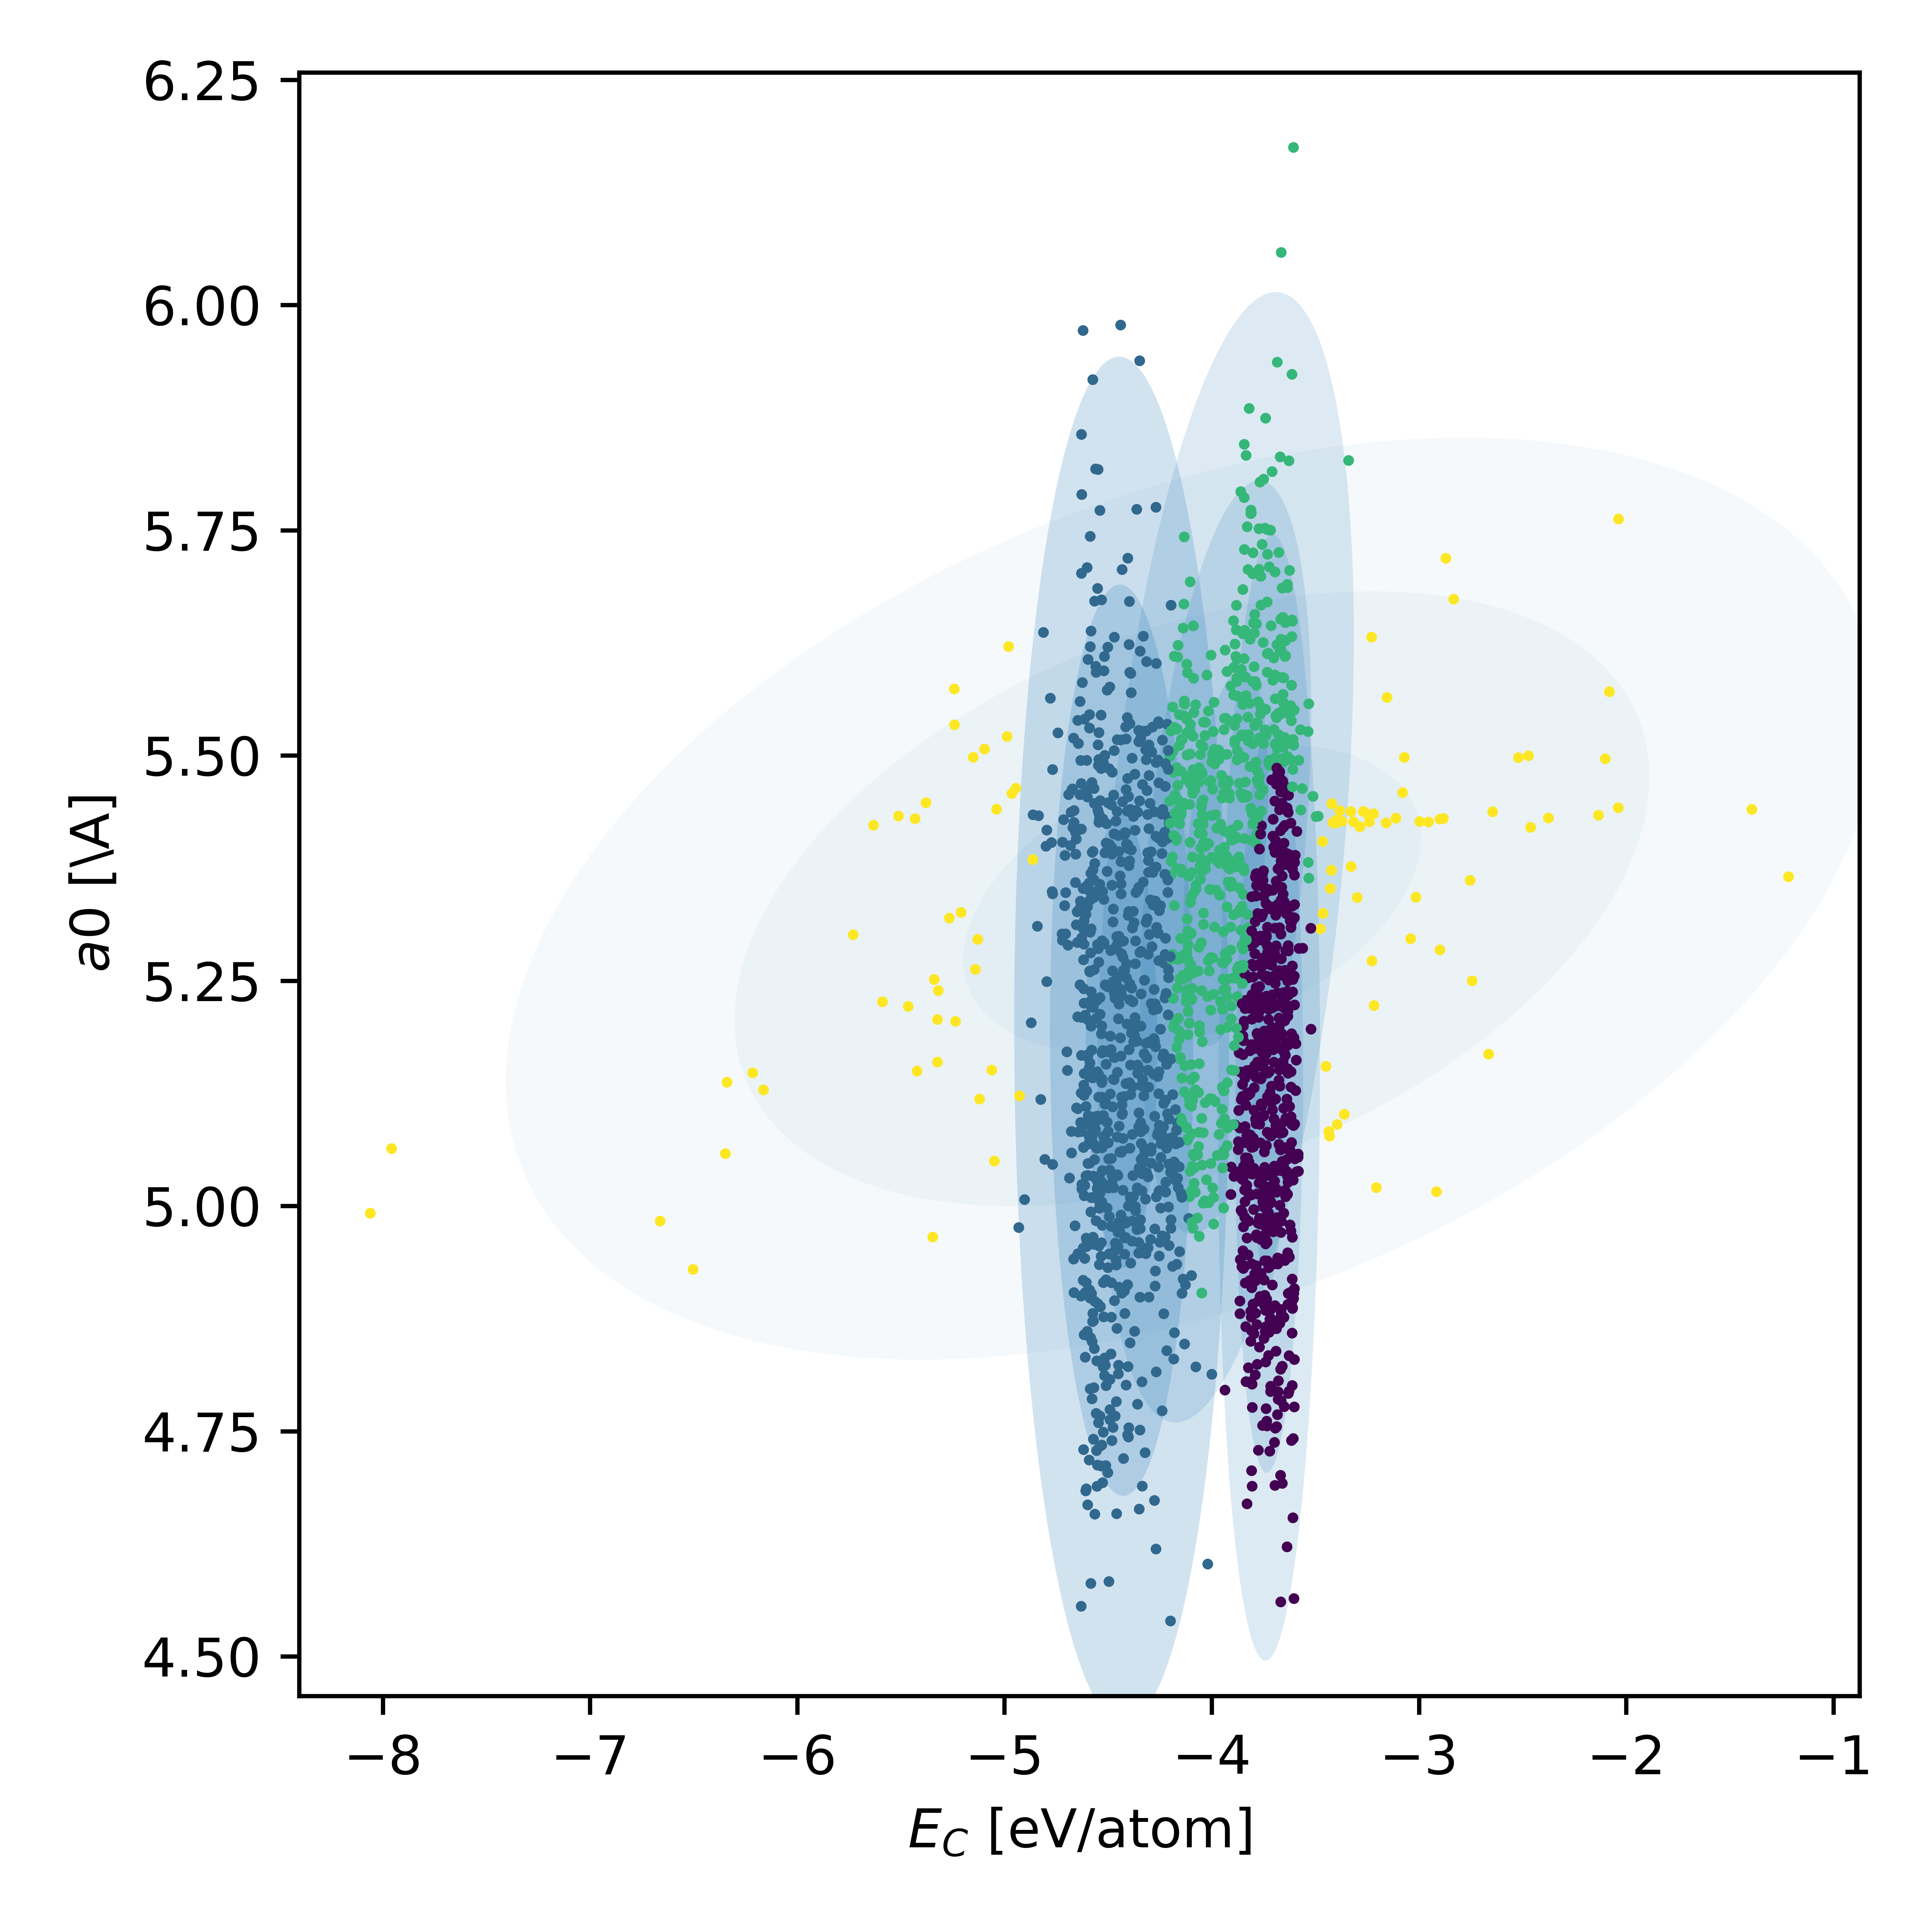
\includegraphics[width=5in]{chapter8/Si_Ec_a0_gmm}
	\caption{Application of the Gaussian mixture model with $K=4$ components.  Ellipses indicating direction and magnitude of the variances are indicated by the grey circles.}
	\label{fig:Si_Ec_a0_gmm}
\end{figure}

\begin{figure}[hbt]
	\centering
	\captionsetup{justification=centering,margin=1in}
	\includegraphics[width=5in]{chapter8/gmm_parallel_plot}
	\caption{Parallel plot}
	\label{fig:Si_gmm_parallel_plot_2_qoi}
\end{figure}

\subsubsection{A general approach to Gaussian mixture models}

We now generalize the approach from 2D case to an application more generally applicable to the potential development process.  As the size of the Pareto set grows, the selection of a potential becomes more difficult.  A GMM process can help partition the set into subsets each defined by a normal distribution.

It is desirable for clusters in $\theta$-space to produce clusters in $q$-space, so that we can characterize the relationship of parameters to material properties predictions.  If clusters are determined in $\theta$-space, there is no guarantee that each cluster would not produce either disperse or multi-modal predictions in $q$-space.  Likewise, if potentials are by performance in $q$-space, a multi-modal distribution in $\theta$-space would imply degenerate regions of parameter space which produce the predictions in a probabilistic sense.  Rather than determine the indivial Gaussian components by an analysis of either $\theta$-space of $q$-space, we pass both the free parameters and the QOIs into the GMM model to identify clusters which produce a compact ball in both $\theta$-space and $q$-space.

To accomplish this, let us define the different components in Equation \ref{eq:gmm}.  Each data point is represented by a the vector $\bm{x}$,
\begin{equation}
	\label{eq:gmm_input_vector_all}
        \bm{x} = (\theta_1,...,\theta_{N_P},\hat{q}_1,...\hat{q}_{N_Q})
\end{equation}
The mean for each component $k$ ,$\bm{\mu}_k$, has the same shape as $\bm{x}$,
\begin{equation}
	\label{eq:gmm_output_mean_all}
	\bm{\mu} = (\theta_{k,1},...,\theta_{k,N_P},\hat{q}_{k,1},...\hat{q}_{k,N_Q})
\end{equation}
The variance covariance matrix from cluster $k$ then becomes
\begin{equation}
	\label{eq:gmm_output_mean_all}
	\bm{\Sigma}_k
	=
	\left(
	    \begin{array}{c|c}
		    \bm{\Sigma}_{k,\bm{\theta},\bm{\theta}} & \bm{\Sigma}_{k,\bm{\theta},\bm{q}} \\
		    \hline
		    \bm{\Sigma}_{k,\hat{\bm{q}},\bm{\theta}}     & \bm{\Sigma}_{k,\bm{\hat{q}},\bm{\hat{q}}}
	    \end{array}
       \right)
       =
       \left(
	      \begin{array}{ccc|ccc}
		   \Sigma_{k,\theta_1,\theta_1}  & \dots  & \Sigma_{k,\theta_1,\theta_{N_P}}
		  &\Sigma_{k,\theta_1,\hat{q}_1} & \dots  & \Sigma_{k,\theta_1,\hat{q}_{N_Q}} \\
		   \vdots                        & \ddots &
		  &\vdots                        & \ddots & \\
		   \Sigma_{k,\theta_{N_P},\theta_1} &     & \Sigma_{k,\theta_{N_P},\theta_{N_P}}
		  &\Sigma_{k,\theta_{N_P},\hat{q}_1} &     & \Sigma_{k,\theta_{N_P},\hat{q}_{N_Q}} \\
		\hline
		\Sigma_{k,\hat{q}_{N_Q},\theta_{N_P}}  & \dots  & \Sigma_{k,\hat{q}_1,\theta_{N_P}}
	       &\Sigma_{k,\hat{q}_1,\hat{q}_1} & \dots  & \Sigma_{k,\hat{q}_1,\hat{q}_{N_Q}} \\
		\vdots                        & \ddots &
	       &\vdots                        & \ddots & \\
		\Sigma_{k,\hat{q}_{N_Q},\theta_1} &     & \Sigma_{k,\hat{q}_1,\theta_1}
	       &\Sigma_{k,\hat{q}_{N_Q},\hat{q}_1} &     & \Sigma_{k,\hat{q}_{N_Q},\hat{q}_{N_Q}}
	      \end{array}
       \right)
\end{equation}
where
$\Sigma_{k,\bm{\theta}, \bm{\theta}}$ is the covariance matrix for the parameters,
$\Sigma_{k,\hat{\bm{q}}, \hat{\bm{q}}}$ is the covariance matrix for the prediction of the parameters, and
$\Sigma_{k,\hat{\bm{q}}, \bm{\theta}}$ contains the covariance relationships between elements of $\hat{\bm{q}}$ and $\bm{\theta}$.

We evaluate GMM models for a large range of possible components ($1 \leq K \leq 100$) and calculate the AIC and BIC for each $K$.  The number of components $K$ are determined using the same AIC and BIC criteria used in the 2D case with results shown in
Figure \ref{fig:Si_aic_bic_all}.  As expected with IC analysis, the AIC estimates a more coarse grained model ($\argmin_K(\text{AIC}_K) = 7$) and the BIC demands a greater number of components ($\argmin_K{\text(BIC)_K} = 57$).
A more coarse grained model here is selected to simplify the analysis with $K=10$, the weights and components for each model are indicated in Table \ref{tbl:sw_all_gmm}.

The structure $\bm{\mu}_k$ can be divided into $\bm{\mu}_{k,\bm{\theta}}$ and $\bm{\mu}_{k,\hat{\bm{q}}}$ which for each cluster $k$ provides the mean in both parameter space and QOI space.
From $\bm{\Sigma}_k$, the $\bm{\Sigma}_{k,\bm{\theta}, \bm{\theta}}$ and $\bm{\Sigma}_{k,\hat{\bm{q}}, \hat{\bm{q}}}$ blocks select the covariance matrices for the paramters and predicted properties, respectively.
Table \ref{tbl:sw_all_gmm_parameters} contains the mean ($\mu$) and standard deviation ($\sigma$) for the parameters in each representative distribution.  Table \ref{tbl:sw_all_gmm_qois} contains the mean ($\mu$) and standard deviation ($\sigma$) for the QOIs for each representative normal distribution.


\begin{figure}[hbt]
	\centering
	\captionsetup{justification=centering,margin=1in}
	\includegraphics[width=5in]{chapter8/aic_bic_all}
	\caption{AIC and BIC}
	\label{fig:Si_aic_bic_all}
\end{figure}

\begin{table}[ht]
	\centering
	\caption{Information for each cluster, $k$  for a full gmm model consisting of the $E_c$ and $a_0$ components along with weighting $\phi$.}
	\label{tbl:sw_all_gmm}
	\begin{tabular}{c c c}
    \hline
    id & $\phi$ & N\\
    \hline
    0 & 0.0110 & 22\\
    1 & 0.1644 & 328\\
    2 & 0.0267 & 53\\
    3 & 0.1897 & 380\\
    4 & 0.1599 & 325\\
    5 & 0.0105 & 21 \\
    6 & 0.0369 & 74 \\
    7 & 0.2124 & 427 \\
    8 & 0.0646 & 124 \\
    9 & 0.1238 & 2 \\
    \hline
  \end{tabular}
\end{table}

\begin{table}[ht]
	\centering
	\caption{QOI information for each constituent distribution, $k$, in the full GMM model.  The $\mu$ and $\sigma$ are provided for each $k$.}
  \label{tbl:sw_all_gmm_parameters}
  \begin{tabular}{ccccccccccc}
    \hline
    $k$ & & $\epsilon$ & $\sigma$ & $a$ & $\lambda$ & $\gamma$ & $A$ & $B$ & $p$ & $q$\\
    \hline
    0 & $\mu$     & 2.1351 & 2.3293 & 1.6766 & 28.5357 & 0.8505 &  9.7152 & 0.5807 & 4.0951 & 0.8467\\
      & $\sigma$  & 0.0682 & 0.2669 & 0.1521 &  7.7997 & 0.1493 &  2.6653 & 0.2228 & 0.9456 & 0.3747\\
    1 & $\mu$     & 2.1490 & 1.9969 & 1.8311 & 25.4190 & 1.5878 &  9.9049 & 0.8331 & 3.6544 & 0.5476\\
      & $\sigma$  & 0.0483 & 0.1617 & 0.1310 &  5.7093 & 0.2308 &  2.2902 & 0.1882 & 0.5614 & 0.3108\\
    2 & $\mu$     & 2.1482 & 1.8758 & 1.8756 & 25.4777 & 1.0569 &  8.3311 & 0.7488 & 3.4368 & 0.5520\\
      & $\sigma$  & 0.0410 & 0.2431 & 0.1961 &  6.7885 & 0.1943 &  2.2901 & 0.2423 & 0.6626 & 0.3784\\
    3 & $\mu$     & 2.1561 & 1.9544 & 1.6951 & 25.9161 & 1.7207 & 13.9368 & 0.8124 & 3.6680 & 0.5712\\
      & $\sigma$  & 0.0448 & 0.1760 & 0.1372 &  6.1449 & 0.3639 &  3.5159 & 0.2045 & 0.6931 & 0.3485\\
    4 & $\mu$     & 2.1491 & 2.1281 & 1.7072 & 24.9994 & 1.9443 & 12.1992 & 0.7337 & 3.5037 & 0.5780\\
      & $\sigma$  & 0.0518 & 0.1678 & 0.1240 &  5.7167 & 0.3621 &  3.4780 & 0.1711 & 0.7115 & 0.3561\\
    5 & $\mu$     & 2.1534 & 2.1774 & 1.8049 & 24.6114 & 1.2441 &  9.7888 & 0.6525 & 3.7626 & 0.7401\\
      & $\sigma$  & 0.0459 & 0.2845 & 0.2144 &  4.9739 & 0.2580 &  5.1655 & 0.2673 & 0.8637 & 0.3980\\
    6 & $\mu$     & 2.1519 & 1.8270 & 1.7388 & 25.5017 & 1.5188 & 13.5491 & 0.8534 & 3.6855 & 0.5233\\
      & $\sigma$  & 0.0401 & 0.1428 & 0.1363 &  5.0800 & 0.4539 &  4.1506 & 0.2208 & 0.6263 & 0.3326\\
    7 & $\mu$     & 2.1476 & 2.0407 & 1.7857 & 26.4184 & 1.1863 & 10.5462 & 0.7723 & 3.6551 & 0.6172\\
      & $\sigma$  & 0.0483 & 0.1930 & 0.1426 &  5.1799 & 0.1745 &  2.7306 & 0.1956 & 0.6134 & 0.3709\\
    8 & $\mu$     & 2.1552 & 2.1884 & 1.7455 & 24.3617 & 1.6889 & 11.6354 & 0.7398 & 3.5336 & 0.6545\\
      & $\sigma$  & 0.0575 & 0.3587 & 0.2754 &  7.1845 & 0.4994 &  4.4585 & 0.3302 & 0.7927 & 0.3982\\
    9 & $\mu$     & 2.1468 & 1.9670 & 1.8592 & 27.0576 & 1.0078 &  9.5202 & 0.8099 & 3.6848 & 0.6391\\
      & $\sigma$  & 0.0513 & 0.1709 & 0.1485 &  4.9628 & 0.1745 & 2.9529 & 0.1818 & 0.6379 & 0.3468\\
    \hline
  \end{tabular}
\end{table}

\begin{table}[ht]
	\centering
	\caption{Parameter information for each constituent distribution, $k$, in the full GMM model.  The $\mu$ and $\sigma$ are provided for each $k$}
  \label{tbl:sw_all_gmm_qois}
  \begin{tabular}{ccccccccc}
    \hline
    $k$ & & $E_C$ & $a0$ & $c_{11}$ & $c_{12}$ & $c_{44}$ & $B$ & $E_v$\\
        & & eV/atom & \AA & GPa & GPa & GPa & GPa & eV \\
    \hline
    0 & $\mu$     & -4.2055 & 5.4118 & 307.8981 & 32.6633 & 137.1558 & 124.4082 & 4.1974\\
     & $\sigma$   & 0.4038 & 0.1788 & 29.8008 & 37.9242 & 12.4975 & 21.3103 & 0.4044\\
    1 & $\mu$     & -4.0628 & 5.3496 & 133.2494 & 98.4785 & 30.5936 & 110.0688 & 4.0628\\
     & $\sigma$   & 0.3429 & 0.1804 & 26.3126 & 26.7241 & 11.3819 & 25.7962 & 0.3429\\
    2 & $\mu$     & -3.9872 & 4.9025 & 141.8443 & -15.6858 & 75.2049 & 36.8243 & 3.9836\\
     & $\sigma$   & 0.3966 & 0.2342 & 38.4908 & 18.0676 & 11.3542 & 14.7759 & 0.3963\\
    3 & $\mu$     & -4.0820 & 5.0081 & 129.9131 & 62.6440 & 57.2602 & 85.0670 & 4.0820\\
     & $\sigma$   & 0.3759 & 0.0822 & 24.9165 & 24.3370 & 13.0931 & 23.1579 & 0.3759\\
    4 & $\mu$     & -3.9786 & 5.3708 & 135.8375 & 121.2139 & 13.8574 & 126.0884 & 3.9786\\
     & $\sigma$   & 0.3800 & 0.1216 & 25.2843 & 22.3983 & 11.1543 & 22.7184 & 0.3800\\
    5 & $\mu$     & -4.5323 & 5.2940 & 159.4287 & 49.0808 & 71.8973 & 85.8634 & 3.6552\\
     & $\sigma$   & 1.7752 & 0.2127 & 32.4540 & 22.2257 & 17.1648 & 23.9528 & 1.7244\\
    6 & $\mu$     & -4.1263 & 4.7881 & 100.8331 & -1.9028 & 71.9410 & 32.3425 & 4.0772\\
     & $\sigma$   & 0.3745 & 0.0921 & 17.8274 & 11.3283 & 11.3778 & 10.9795 & 0.3816\\
    7 & $\mu$     & -4.1075 & 5.2920 & 166.8931 & 72.5505 & 69.1024 & 103.9980 & 4.1075\\
     & $\sigma$   & 0.5248 & 0.2041 & 35.2261 & 26.5453 & 15.3744 & 27.3971 & 0.5248\\
    8 & $\mu$     & -4.1252 & 5.3739 & 123.7958 & 89.8818 & 26.4300 & 101.1865 & 4.1252\\
     & $\sigma$   & 0.3735 & 0.2946 & 39.4293 & 39.0031 & 29.7312 & 35.5491 & 0.3734\\
    9 & $\mu$     & -4.0385 & 5.2610 & 209.4494 & 26.7454 & 99.4384 & 87.6467 & 4.0385\\
     & $\sigma$   & 0.4629 & 0.2546 & 52.3615 & 26.9835 & 21.0676 & 28.7038 & 0.4629\\
    \hline
  \end{tabular}
\end{table}

\subsection{Possible Applications}

\subsubsection{More Efficient KDE Sampling}
In the Pareto optimization process, the Pareto surface is estimated by evolving a kernel density esimate (KDE).  Since the KDE is non-parametric, it overcomes the problems with the strong assumptions with the parametric distribution.  Particularly the assumption that underlying distribution should be unimodal distribution.  The KDE is not without its limiations. the KDE assumes that variance and covaraince are homoskedastic since the same bandwidth matrix is applied across the range of possible parameterizations.

The GMM models partitions the parameter space into populations, which are defined by location and the direction and magnitude of a dispersion.  As a result, each cluster $K$ can be defined by a single bandwidth matrix, since the population $k$ is dispersed by $\bm{\Sigma}_{k,\Theta,\Theta}$ by construction.

After convergence is met, the potential developer may want to identify more potentials in a region of interest.  The GMM models allows the developer to isolate and eliminate certain regions from consideration.  Since the probability density of $\bm{\theta}$ is localized to a particular region, the sampling intensity would increase easing the sampling demands to find a new Pareto optimal potential.

If $k$ is chosen to be sufficiently high, the variance of the parameters as well as the predicted QOI values becomes reduced, and the Normal distribution specified in parameter space could be used for feed forward Bayesian UQ methodologies since the calculation of the analytical form of likelihood function for the Normal distribution known.

\subsubsection{Algorithmic Subselection of Potentials}

Unlike Chapter \ref{ch:ionic_MgO}, our options here are no longer individual potentials but described by a normal probability distribution for each constituitive options.  For an empirical interatomic potentials where the mean $\mu_{k,\hat{\bm{q}}}$ is sufficently close to the the target QOI values.  A one sample Hotelling's $t$-squared  ($T^2$)\cite{hotelling1931_t2} could be used. However, since none of the components are likely to contain the vector $\bm{q}$, having $p$-values near to $1$.

Instead we construct a series of Student's $t$-tests for each $q_i$.  For each cluster $k$ and QOI $i$, we test if $\bm{q}_i$ is in the distribution defined by $\mu_i = \mu_{k,q_i}$ and $\sigma = \Sigma_{k,q_i,q_i}$, where the  mean $\mu_{k,q_i}$ and the variance components $\Sigma_{k,q_i,q_i}$ are individual components from $\bm{\mu}_{k,q}$ (see Table \ref{tbl:sw_all_gmm_qois}.
The calculated values for the $t$-test values for each of the QOI and Gaussian components is listed in Table \ref{tbl:sw_all_gmm_ttest}.

The last column of Table \ref{tbl:sw_all_gmm_qois} is an aggregate metric, which is here now derived.  The $p$-value can be interpreted as the probability that $\mathbb{P}[q_i\notin \hat{Q}_i^*]$ for each component $i$.  If each component $i$ is assumed to be independent, then the
\begin{align}
  \mathbb{P}[\bm{q} \in \hat{\bm{Q}}]
  =
  & 1 - \prod_i^{N_Q} \left(1 - \mathbb{P}[q_i \notin \hat{Q}_i^*]\right) \\
  & 1 - \prod_i^{N_Q} \mathbb{P}[q_i \in \hat{Q}_i^*] \\
  \mathbb{P}[\bm{q} \notin \hat{\bm{Q}}]
  &= \prod_i^{N_Q} \mathbb{P}[q_i \in \hat{Q}_i^*]
  \label{eq:aggregate_t_test}
\end{align}
which can be interpreted as a aggregate $t$-test for uncorrelated components.

\begin{table}[ht]
	\centering
	\caption{The $p$-value type scoring for each constituent distribution, $k$, in the full GMM model. Each $q$ is tested to determine is in the normal distribution, $N(\bm{\mu}_{k,q}, \bm{\Sigma}_{k,q})$}
	\label{tbl:sw_all_gmm_ttest}
	\begin{tabular}{ccccccccc}
		\hline
		$k$ & $E_C$ & $a0$ & $c_{11}$ & $c_{12}$ & $c_{44}$ & $B$ & $E_v$ & total \\
		    & eV/atom & \AA & GPa & GPa & GPa & GPa & eV & \\
		\hline
		0 & 0.0046 & 0.2843 & 0.4365 & 0.4913 & 0.3572 & 0.4777 & 0.0001 & 0.9314\\
		1 & 0.0000 & 0.0068 & 0.4811 & 0.4807 & 0.3515 & 0.4934 & 0.0000 & 0.9121\\
		2 & 0.0000 & 0.0000 & 0.4935 & 0.4036 & 0.4852 & 0.3879 & 0.0073 & 0.9055\\
		3 & 0.0001 & 0.0000 & 0.4768 & 0.4991 & 0.4472 & 0.4896 & 0.0003 & 0.9261\\
		4 & 0.0000 & 0.0000 & 0.4812 & 0.4546 & 0.2975 & 0.4791 & 0.0044 & 0.8969\\
		5 & 0.4876 & 0.0013 & 0.4975 & 0.4880 & 0.4890 & 0.4909 & 0.4926 & 0.9826\\
		6 & 0.0002 & 0.0000 & 0.4188 & 0.3038 & 0.4752 & 0.2902 & 0.0005 & 0.8494\\
		7 & 0.0289 & 0.0005 & 0.4997 & 0.4952 & 0.4816 & 0.4973 & 0.0327 & 0.9382\\
		8 & 0.0001 & 0.2590 & 0.4892 & 0.4932 & 0.4758 & 0.4993 & 0.0001 & 0.9497\\
		9 & 0.0029 & 0.0046 & 0.4937 & 0.4796 & 0.4825 & 0.4945 & 0.0204 & 0.9330\\
		\hline
	\end{tabular}
\end{table}

The results of each $t$-test provides a metric to assess the performance of each cluster $k$ with respect to a QOI $i$; Equation \ref{eq:aggregate_t_test} provides an aggregate $p$-value.  First, we note that since the $t$-test is based upon a cumulative distribution function of Student's $t$-distribution, then it is monotonically increasing with respect to $|epsilon|_i$ and satisfies the ordinality conditions for loss function imposed in Chapter \ref{ch:potential_development}.  Then Equation \ref{eq:aggregate_t_test} can be interpreted as a probabilistic cost function, which can be applied to ensembles of potentials.
Minimizing Equation \ref{eq:aggregate_t_test} maximizes the probability that $\bm{q} \in \hat{\bm{Q}}^*$, and solves the optimization problem.

Inspection of the aggregate performance of each potential shows high values which infers what we already know; it is not possible to minimize $|epsilon_i|$ for all $i$ simultaneously due to the performance tradeoffs in the formalism of our interatomic potential.  Prediction for elements of the elastic tensor $c_{11}$, $c_{12}$, and $c_{44}$ is generally poor; the same analysis applies to the bulk modulus $B$.  For elastic properties and aggregate performance, the performance metric is of the same order of magnitude, and we should not use the metric as a discriminating factor.

  However, the $t$-test does allow us to descriminate performance of the of the remaining QOIs.  Let us use $p > 0.01$ as a discriminating inequality.  For the cohesive energy, $E_c$, clusters $5$ and $7$ have poor performance.  For predictions of the lattice parameter $a_0$, clusters $0$ and $8$ have poor performance.  For the vacancy formation energy $E_v$, clusters $5$, $7$, and $9$ have poor performance.  Our remaining clusters then become $k = \{1,2,3,4,6,8\}$.
